\newcommand{\ds}{\displaystyle}
\section{Image analysis}
\begin{slide}\slidetitle{Image analysis}
\tableofcontents[sectionstyle=show/hide,subsectionstyle=show/shaded/hide]

\end{slide}

\subsection{Computer Vision and Classification}\begin{slide}\slidetitle{The $k$-nearest-neighbor method}

The {\em $k$-nearest-neighbor} (knn) procedure has been used in data
analysis and machine learning communities as a quick way to classify objects into predefined groups.

\vs\pause This approach requires a training dataset where both the class $y$ and the vector $\mathbf{x}$
of characteristics (or covariates) of each observation are known. 

\end{slide}\begin{slide}\slidetitle{The $k$-nearest-neighbor method}

The training dataset $\left(y_i,\mathbf{x}_i\right)_{1\le i\le n}$ is used by the $k$-nearest-neighbor procedure to predict the value
of $y_{n+1}$ given a new vector of covariates $\mathbf{x}_{n+1}$ in a very rudimentary manner. 

\vs\pause \BrickRed{The predicted value of $y_{n+1}$ is simply the most frequent class found amongst the $k$ nearest
neighbors of $\mathbf{x}_{n+1}$ in the set $(\mathbf{x}_i)_{1\le i\le n}$.}

\end{slide}\begin{slide}\slidetitle{The $k$-nearest-neighbor method}

The classical knn procedure does not involve much calibration and requires no statistical modeling at all!

\vs\pause \BrickRed{There exists a Bayesian reformulation.}

\end{slide}\begin{slide}\slidetitle{{\bfseries vision} dataset (1)}

\RedOrange{{\sf vision}}: $1373$ color pictures, described by $200$ variables rather than by
the whole table of $500\times 375$ pixels

\vs\pause Four classes of images: 
class $C_1$ for motorcycles, class $C_2$ for bicycles, class $C_3$ for humans
and class $C_4$ for cars

\end{slide}\begin{slide}\slidetitle{{\bfseries vision} dataset (2)}

Typical issue in computer vision problems: build a classifier to identify a
picture pertaining to a specific topic without human intervention

\vs\pause We use about half of the images ($648$ pictures) to construct the training dataset and we save the
$689$ remaining images to test the performance of our procedures. 

\end{slide}\begin{slide}\slidetitle{{\bfseries vision} dataset (3)}

\begin{figure}
\centerline{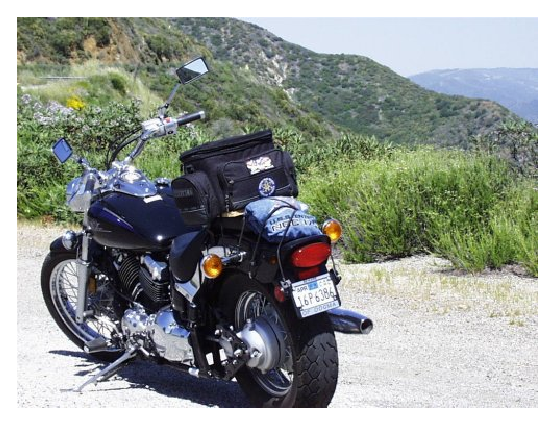
\includegraphics[width=4cm,height=2.5cm]{figures/moto.eps}\quad
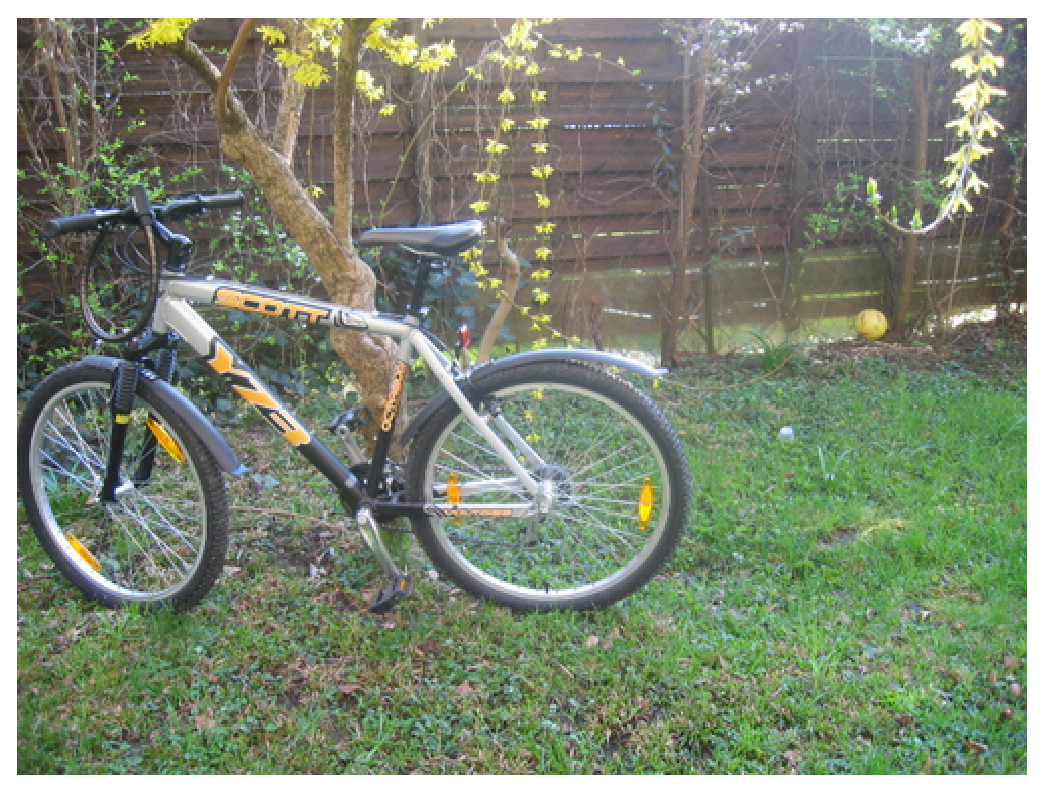
\includegraphics[width=4cm,height=2.5cm]{figures/bike.eps}}
\medskip
\centerline{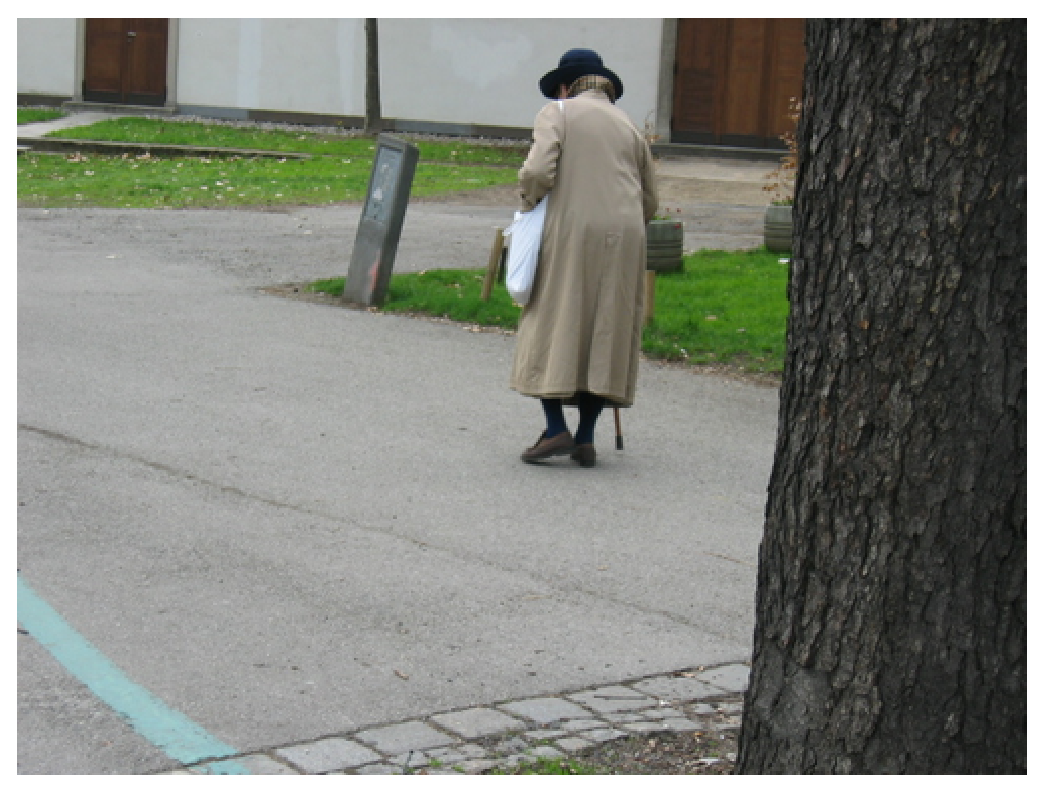
\includegraphics[width=4cm,height=2.5cm]{figures/people.eps}\quad
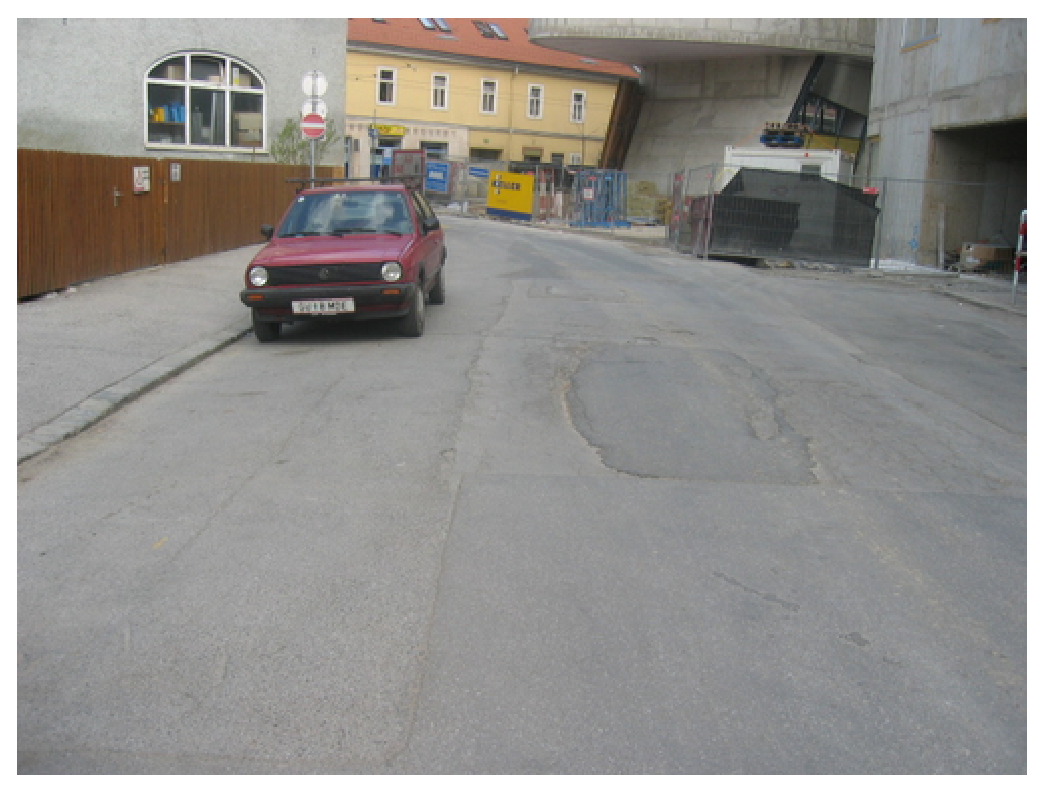
\includegraphics[width=4cm,height=2.5cm]{figures/car.eps}}
\end{figure}

\end{slide}\begin{slide}\slidetitle{A probabilistic version of the knn methodology (1)}

{\em Symmetrization} of the neighborhood relation: If $\mathbf{x}_i$ belongs to the $k$-nearest-neighborhood
of $\mathbf{x}_j$ and if $\mathbf{x}_j$ does not belong to the $k$-nearest-neighborhood of $\mathbf{x}_i$, 
the point $\mathbf{x}_j$ is added to the set of neighbors of $\mathbf{x}_i$

\vs\pause
\RedOrange{{\bf Notation:}} $i\sim_k j$

\vs\pause The transformed set of neighbors is then called the {\em symmetrized
$k$-nearest-neighbor system.} 

\end{slide}\begin{slide}\slidetitle{A probabilistic version of the knn methodology (2)}

\begin{figure}
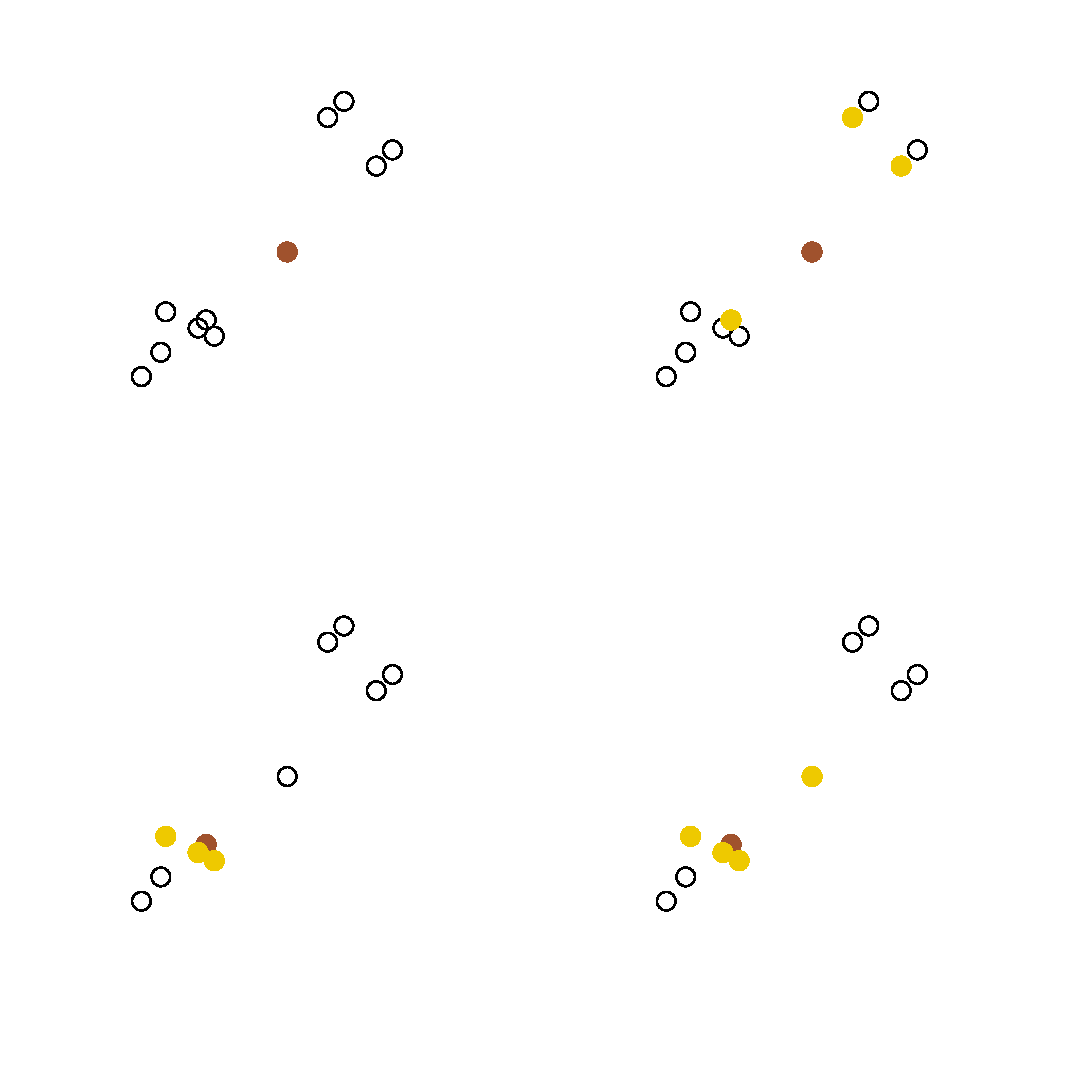
\includegraphics[width=.7\textwidth]{figures/neighbR.eps}
\end{figure}

\end{slide}\begin{slide}\slidetitle{A probabilistic version of the knn methodology (3)}

$$
\mathbb{P}(y_i=C_j|\mathbf{y}_{-i},\mathbf{X},\beta,k)=\frac{\ds \exp\left(\beta \sum_{\ell\sim_k i}
\mathbb{I}_{C_j}(y_\ell)\bigg/N_k \right)}
{\ds \sum_{g=1}^G\exp\left(\beta \sum_{{\ell\sim_k i}} \mathbb{I}_{C_g}(y_\ell)\bigg/N_k \right)}\,,
$$
$N_k$ being the average number of neighbours over all $x_i$'s, $\beta>0$ and
$$
\mathbf{y}_{-i}=\left(y_1,\ldots,y_{i-1},y_{i+1},\ldots,y_n\right)\quad \mbox{and}
\quad \mathbf{X}=\{\mathbf{x}_1,\ldots,\mathbf{x}_n\}\,.
$$

\end{slide}\begin{slide}\slidetitle{A probabilistic version of the knn methodology (4)}

\begin{itemize}
\item $\beta$ grades the influence of the prevalent neighborhood class ;

\item \pause the probabilistic knn model is conditional on the covariate matrix $\mathbf{X}$ ; 

\item \pause the frequencies $n_1/n,\ldots,n_G/n$ of the classes within the
training set are representative of the marginal
probabilities $p_1=\mathbb{P}(y_i=C_1),\ldots,p_G=\mathbb{P}(y_i=C_G)$: 
\end{itemize}

\vs \pause If the marginal probabilities $p_g$ are known and different from $n_g/n$ 
$\Longrightarrow$ reweighting the various classes according to their true frequencies

\end{slide}\begin{slide}\slidetitle{Bayesian analysis of the knn probabilistic model}

From a Bayesian perspective, given a prior distribution $\pi(\beta,k)$ with support
$[0,\beta_{\max{}}]\times\{1,\ldots,K\}$, the marginal predictive distribution of $y_{n+1}$ is
\begin{align*}
\mathbb{P}(y_{n+1}=C_j|&\mathbf{x}_{n+1},\mathbf{y},\mathbf{X})= \\
 &\sum_{k=1}^K\int_0^{\beta_{\max}} \mathbb{P}(y_{n+1}=C_j|
\mathbf{x}_{n+1},\mathbf{y},\mathbf{X},\beta,k)\pi(\beta,k|\mathbf{y},\mathbf{X})\,\text{d}\beta\,,
\end{align*}
where $\pi(\beta,k|\mathbf{y},\mathbf{X})$ is the posterior distribution given the training dataset
$(\mathbf{y},\mathbf{X})$. 

\end{slide}\begin{slide}\slidetitle{Unknown normalizing constant}

Major difficulty: it is impossible to compute $f(\mathbf{y}|\mathbf{X},\beta,k)$

\vs\pause Use instead the {\em pseudo-likelihood} made of
the product of the full conditionals
$$
\widehat{f}(\mathbf{y}|\mathbf{X},\beta,k) =
\prod_{g=1}^G\, \prod_{y_i=C_g}\, \mathbb{P}(y_i=C_g|\mathbf{y}_{-i},\mathbf{X},\beta,k)\,
$$

\end{slide}\begin{slide}\slidetitle{Pseudo-likelihood approximation}

Pseudo-posterior distribution
$$
\widehat{\pi}(\beta,k|\mathbf{y},\mathbf{X})\propto \widehat{f}(\mathbf{y}|\mathbf{X},\beta,k)\pi(\beta,k)
$$

\vs\pause Pseudo-predictive distribution
\begin{align*}
\widehat{\mathbb{P}}&(y_{n+1}=C_j|\mathbf{x}_{n+1},\mathbf{y},\mathbf{X})= \nonumber \\
  &\sum_{k=1}^K\,\int_0^{\beta_{\max}}\,\mathbb{P}(y_{n+1}=C_j|\mathbf{x}_{n+1},\mathbf{y},
    \mathbf{X},\beta,k)\widehat{\pi}(\beta,k|\mathbf{y},\mathbf{X})\,\text{d}\beta\,.
\end{align*}

\end{slide}\begin{slide}\slidetitle{MCMC implementation (1)}

MCMC approximation is required

\vs\pause Random walk Metropolis--Hastings algorithm

\vs\pause Both $\beta$ and $k$ are updated using random walk proposals:

\vs\pause (i) for $\beta$, logistic tranformation
$$
\beta^{(t)}=\beta_{\max{}}\exp(\theta^{(t)})\big/ (\exp(\theta^{(t)})+1)\,,
$$
in order to be able to simulate a normal random walk on the $\theta$'s, $\tilde\theta\sim\mathcal{N}(\theta^{(t)},\tau^2)$;

\end{slide}\begin{slide}\slidetitle{MCMC implementation (2)}

(ii) for $k$,  we use a uniform proposal on the $r$ neighbors of $k^{(t)}$, namely on $\{ k^{(t)}-r,\ldots,
k^{(t)}-1,k^{(t)}+1, \ldots k^{(t)}+r \}\cap\{1,\ldots,K\}$. 

\vs \pause Using this algorithm, we can thus derive the most likely class
associated with a covariate vector $\mathbf{x}_{n+1}$ from the
approximated probabilities,
$$
\frac{1}{M}\,\sum_{i=1}^M \widehat{\mathbb{P}}\left(y_{n+1}=l|x_{n+1},y,x,(\beta^{(i)},k^{(i)})\right)\,.
$$

\end{slide}\begin{slide}\slidetitle{MCMC implementation (3)}

\begin{figure}
\begin{center}
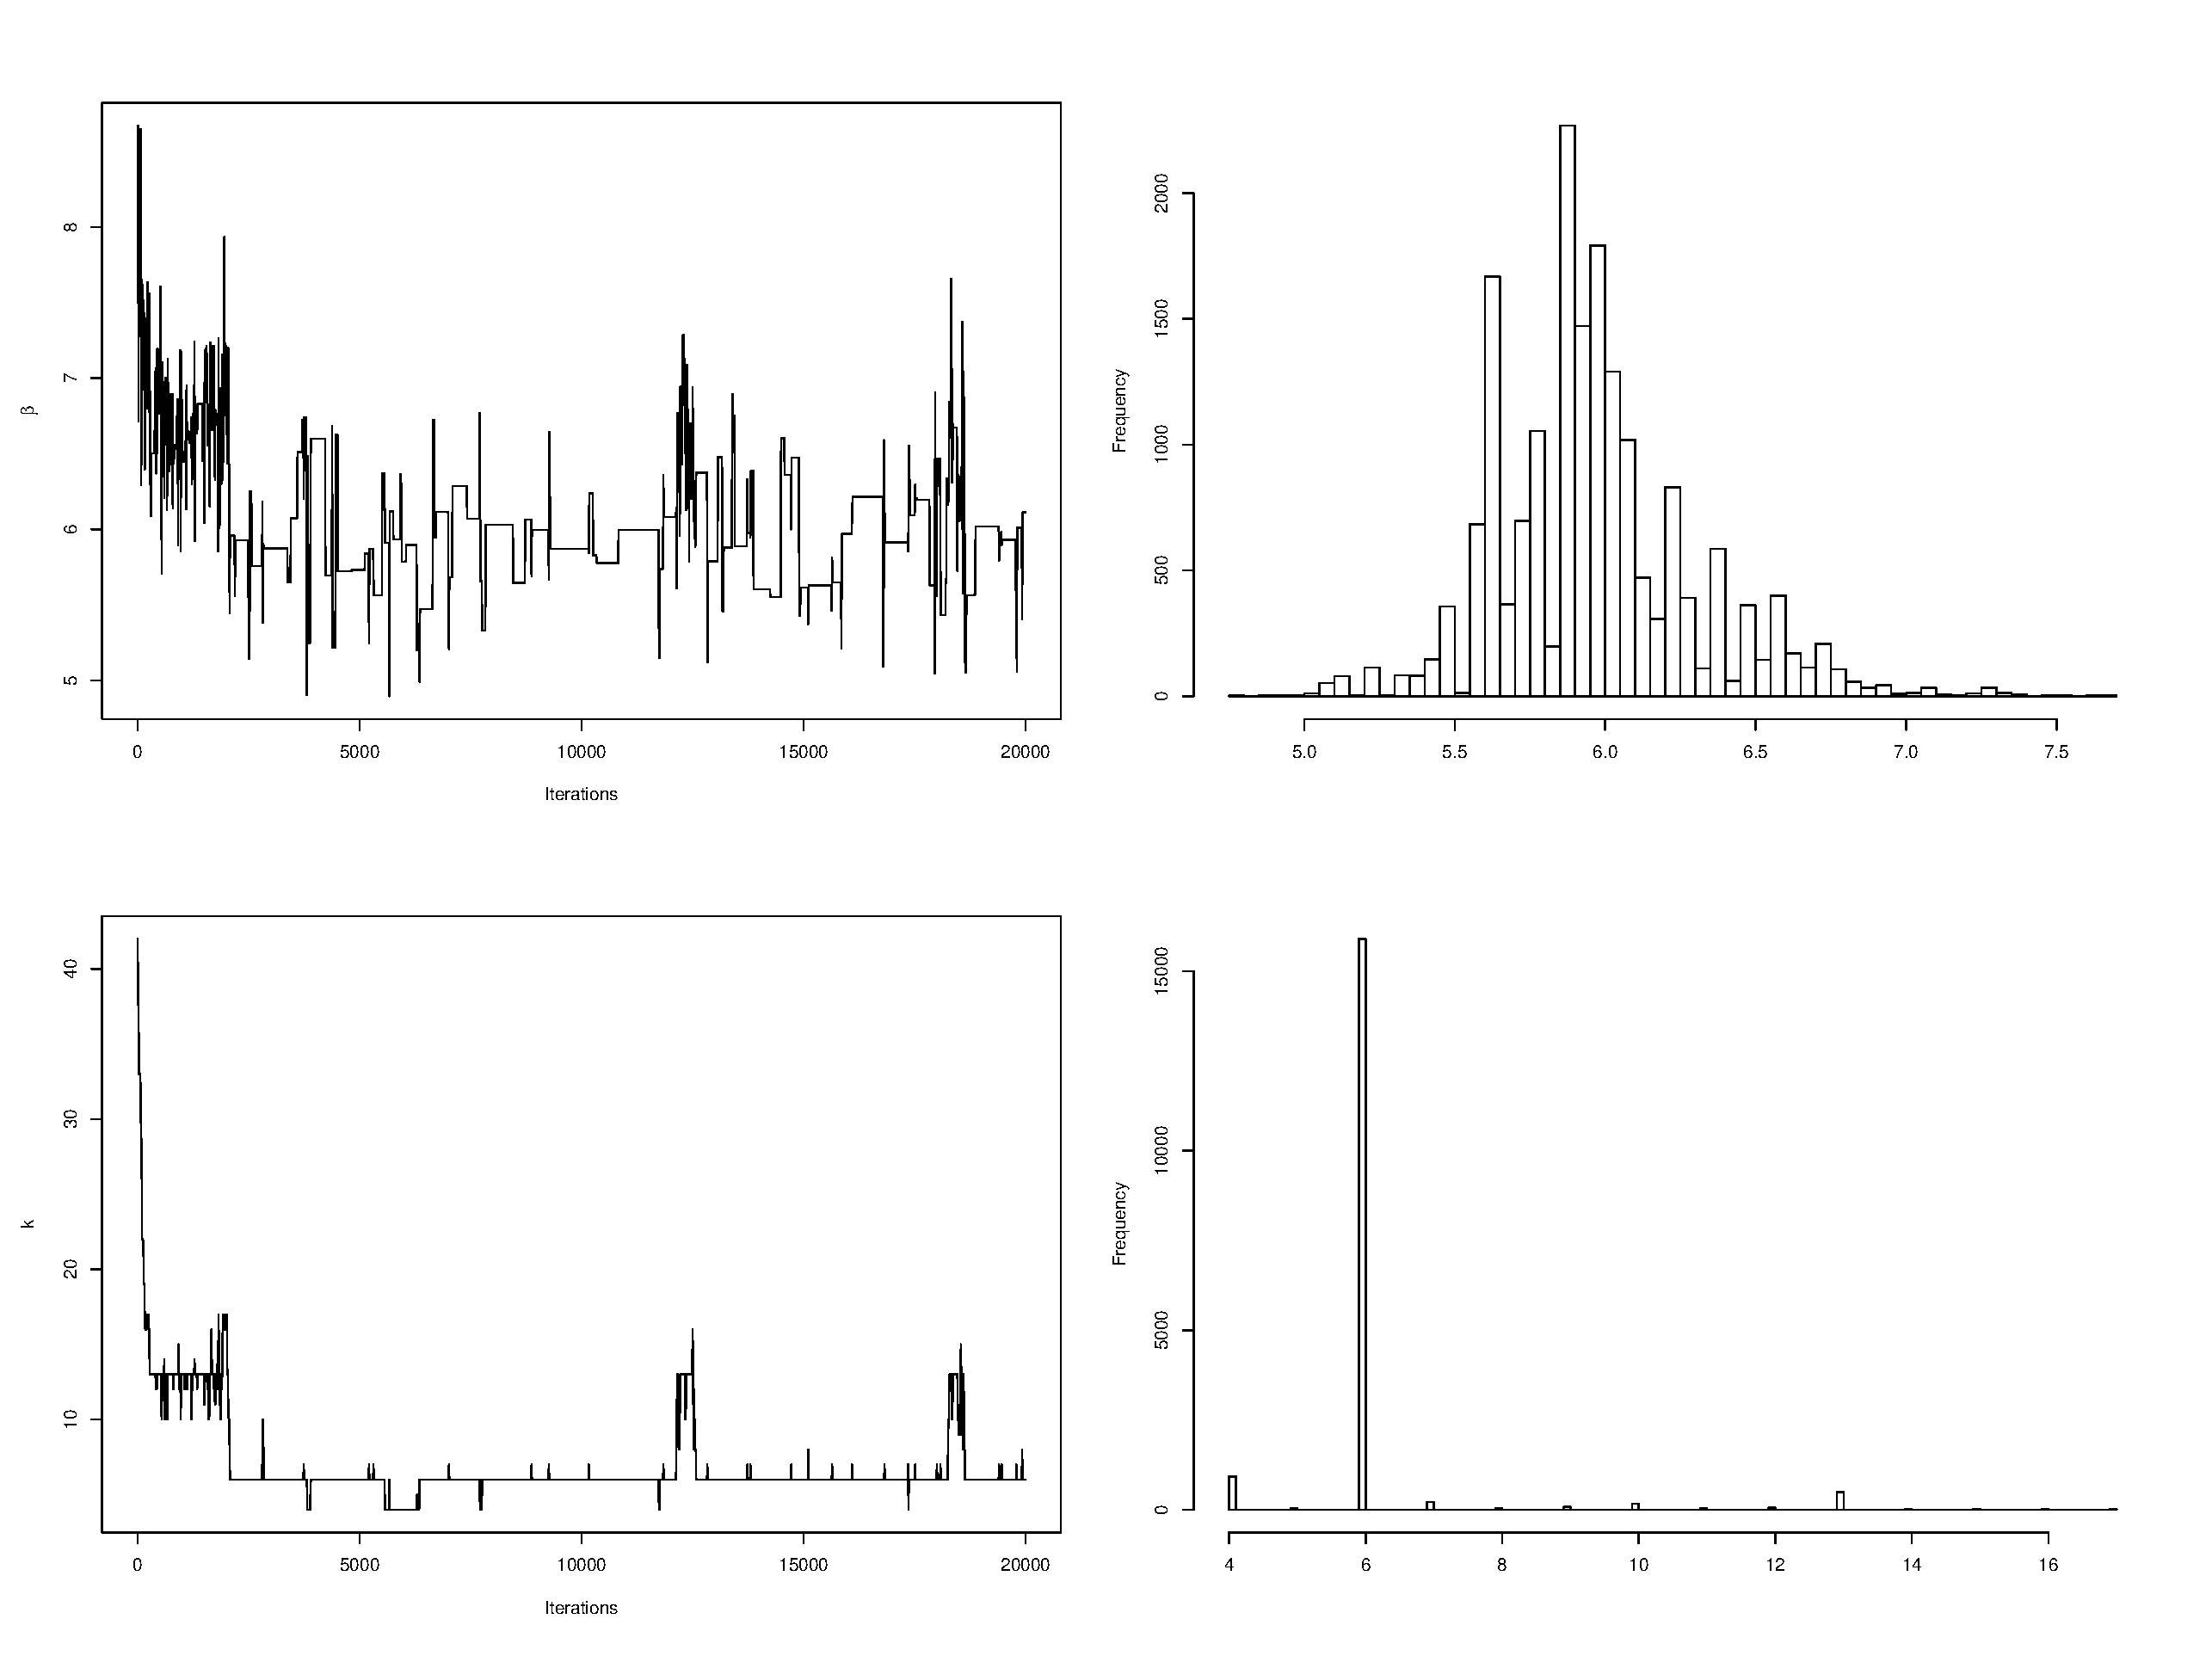
\includegraphics[width=10cm,height=4.5cm]{figures/res2.eps}
\end{center}
\end{figure}

\footnotesize \begin{center}
$\beta_{\max}=15$, $K=83$, $\tau^2=0.05$ and $r=1$ \\
$k$ sequences for the {\sf knn} Metropolis--Hastings $\beta$ 
based on $20,000$ iterations
\end{center}

\end{slide}

\subsection{Image Segmentation}\begin{slide}\slidetitle{Image Segmentation}

This underlying structure of the ``true" pixels is denoted by $\bx$, while the observed image is
denoted by $\by$. 

\vs \pause Both objects $\bx$ and $\by$ are arrays, with each entry of $\bx$ taking a finite number of
values and each entry of $\by$ taking real values. 

\vs \pause \BrickRed{We are interested in the posterior distribution of $\bx$ given $\by$ provided by
Bayes' theorem, $\pi(\bx|\by)\propto f(\by|\bx)\pi(\bx)$.}

\vs \pause The likelihood, $f(\by|\bx)$, describes the link between the observed image and the
underlying classification.

\end{slide}\begin{slide}\slidetitle{{\bfseries Menteith} dataset (1)}

The {\bfseries Menteith} dataset is a $100\times 100$ pixel satellite image of the lake of Menteith.

\vs \pause The lake of Menteith is located in Scotland\index{Scotland}, near Stirling, and offers the
peculiarity of being called ``lake" rather than the traditional Scottish ``loch." 

\end{slide}\begin{slide}\slidetitle{{\bfseries Menteith} dataset (2)}

\begin{figure}
\begin{center}
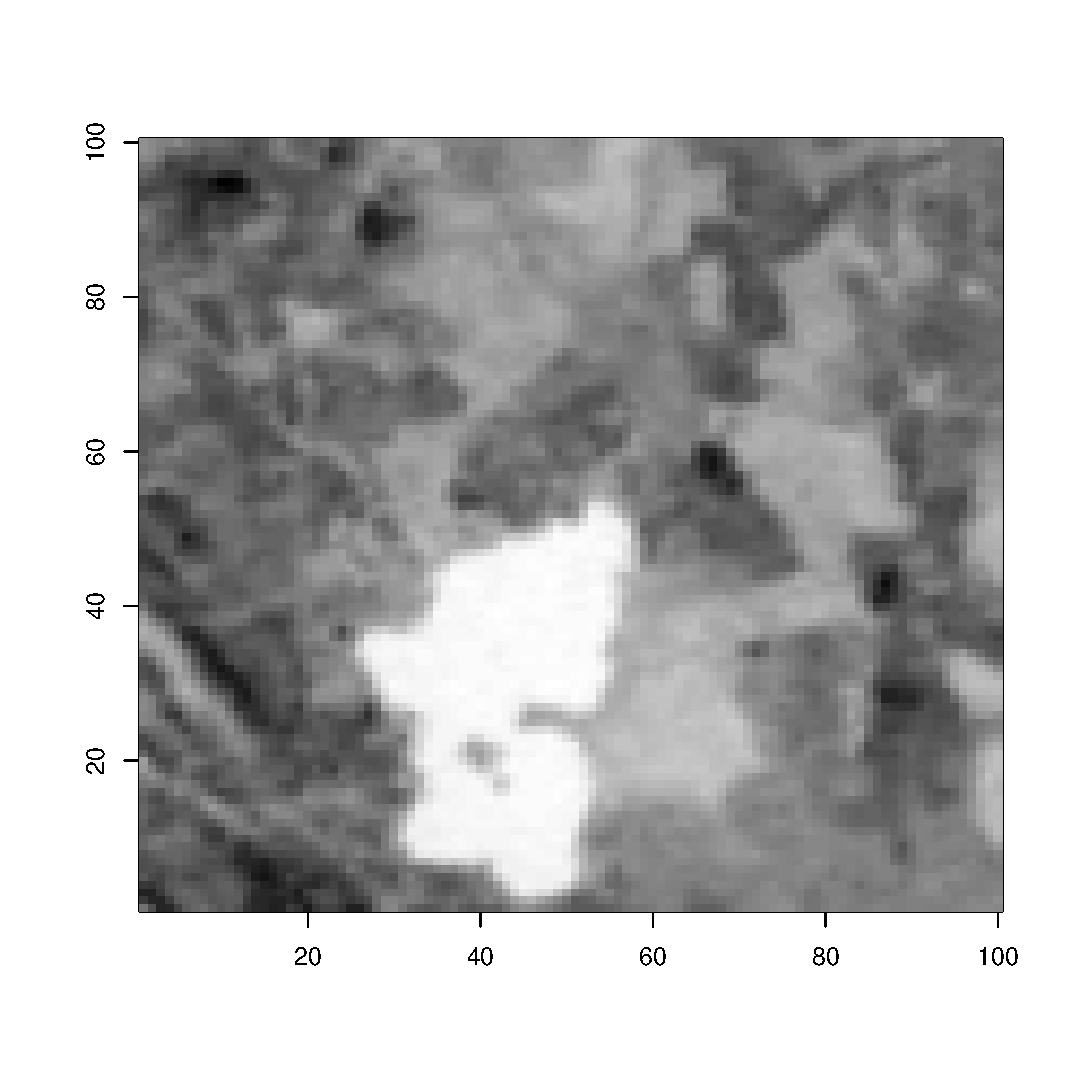
\includegraphics[width=6cm,height=6cm]{figures/menteith.eps}
\end{center}
\end{figure}

\footnotesize \begin{center}Satellite image of the lake of Menteith\end{center}

\end{slide}\begin{slide}\slidetitle{Random Fields}

If we take a lattice $\mathcal{I}$ of sites or pixels in an image, we denote by
$i\in\mathcal{I}$ a coordinate in the lattice.  The neighborhood relation is then denoted by $\sim$. 

\vs \pause A {\em random field} on $\mathcal{I}$ is a random structure indexed by the lattice $\mathcal{I}$, a
collection of random variables $\{x_i;i\in\mathcal{I}\}$ where each
$x_i$ takes values in a finite set $\chi$. 

\end{slide}\begin{slide}\slidetitle{Markov Random Fields}

Let $\bx_{n(i)}$ be the set of values taken by the neighbors of $i$. 

\vs \pause A random field is a {\em Markov random field} (MRF) if the conditional distribution of any pixel given the
other pixels only depends on the values of the neighbors of that pixel; i.e., for $i\in\mathcal{I}$,
$$
\pi(x_i|\bx_{-i})=\pi(x_i|\bx_{n(i)})\,.
$$

\end{slide}\begin{slide}\slidetitle{Ising Models}

If pixels of the underlying (true) image $\bx$ can only take two
colors (black and white, say), $\bx$ is then binary, while $\by$ is
a grey-level image.

\vs \pause We typically refer to each pixel $x_i$ as being {\em foreground}
if $x_i=1$ (black) and {\em background} if $x_i=0$ (white).

\vs \pause We have 
$$
\pi(x_i=j|\bx_{-i})\propto \exp(\beta n_{i,j})\,,\qquad\beta>0\,,
$$
where $n_{i,j}=\sum_{\ell\in n(i)}\mathbb{I}_{x_\ell=j}$ is the
number of neighbors of $x_i$ with color $j$. 

\end{slide}\begin{slide}\slidetitle{Ising Models}

The {\em Ising model} is defined via full conditionals
$$
\pi(x_i=1|\bx_{-i})=\frac{\exp(\beta n_{i,1})}{\exp(\beta n_{i,0})+\exp(\beta n_{i,1})}\,,
$$
\pause and the joint distribution satisfies
$$
\pi(\bx)\propto \exp\left(\beta \sum_{j\sim i} \mathbb{I}_{x_j=x_i}\right)\,,
$$
where the summation is taken over all pairs $(i,j)$ of neighbors.

\end{slide}\begin{slide}\slidetitle{Simulating from the Ising Models}

The normalizing constant of the Ising Model is intractable except for very small lattices $\mathcal{I}$...

\vs \pause \BrickRed{{\bf Direct simulation of $\bx$ is not possible!}}

\end{slide}\begin{slide}\slidetitle{Ising Gibbs Sampler}

\begin{algo}[{\bf Ising Gibbs Sampler}]
\begin{itemize}
\item[ ]Initialization: For $i\in\mathcal{I}$, generate independently
$$
x_i^{(0)}\sim\mathscr{B}(1/2)\,.
$$
\item[ ] Iteration $t$ $(t\ge 1)$:
\begin{enumerate}
\item Generate $\mathbf{u}=(u_i)_{i\in\mathcal{I}}$, a random ordering of the elements of $\mathcal{I}$.
\item For $1\le \ell\le |\mathcal{I}|$, update $n_{u_\ell,0}^{(t)}$ and $n_{u_\ell,1}^{(t)}$, and generate
$$
x_{u_\ell}^{(t)}\sim\mathscr{B}\left\{\frac{\exp(\beta n_{u_\ell,1}^{(t)})}
{\exp(\beta n_{u_\ell,0}^{(t)})+\exp(\beta n_{u_\ell,1}^{(t)})}\right\}\,.
$$
\end{enumerate}
\end{itemize}
\end{algo}

\end{slide}\begin{slide}\slidetitle{Ising Gibbs Sampler (2)}

\begin{figure}
\begin{center}
\includegraphics[width=5cm,height=10cm,angle=270]{figures/gising.eps}
\end{center}
\end{figure}

\footnotesize Simulations from the Ising model with
a four-neighbor neighborhood structure on a $100\times 100$ array after
$1,000$ iterations of the Gibbs sampler: $\beta$ varies in steps of
$0.1$ from $0.3$ to $1.2$.

\end{slide}\begin{slide}\slidetitle{Potts Models}

If there are $G$ colors and if $n_{i,g}$ denotes the number of neighbors of $i\in\mathcal{I}$ with color $g$
$(1\le g\le G)$ (that is, $n_{i,g}=\sum_{j\sim
i}\mathbb{I}_{x_j=g}$)

In that case, the full conditional distribution of $x_i$ is
chosen to satisfy $\pi(x_i=g|\bx_{-i})\propto \exp(\beta n_{i,g})$.

This choice corresponds to the {\em Potts model}, whose joint
density is given by
$$
\pi(\bx)\propto \exp\left(\beta \sum_{j\sim i} \mathbb{I}_{x_j=x_i}\right)\,.
$$

\end{slide}\begin{slide}\slidetitle{Simulating from the Potts Models (1)}

\begin{algo}[{\bf Potts Metropolis--Hastings Sampler}]
\begin{itemize}
\item[] Initialization: For $i\in\mathcal{I}$, generate independently
$$
x_i^{(0)}\sim\mathscr{U}(\{1,\ldots,G\})\,.
$$
\item[] Iteration $t$ $(t\ge 1)$:
\begin{enumerate}
\item Generate $\mathbf{u}=(u_i)_{i\in\mathcal{I}}$ a random ordering of the elements of $\mathcal{I}$.
\item For $1\le\ell\le|\mathcal{I}|$,
\begin{itemize}
\item[] generate
$$
\tilde x_{u_\ell}^{(t)}\sim\mathscr{U}(\{1,x_{u_\ell}^{(t-1)}-1,x_{u_\ell}^{(t-1)}+1,\ldots,G\})\,,
$$
\end{itemize}
\end{enumerate}
\end{itemize}
\end{algo}

\end{slide}\begin{slide}\slidetitle{Simulating from the Potts Models (2)}

\begin{algo}[continued]
\begin{itemize}
\item[] compute the $n_{u_l,g}^{(t)}$ and
$$
\rho_l=\left\{ \exp(\beta n_{u_\ell,\tilde x}^{(t)})/\exp(\beta n_{u_\ell,x_{u_\ell}}^{(t)})\right\} \wedge 1\,,
$$
\item[] and set $x_{u_\ell}^{(t)}$ equal to $\tilde x_{u_\ell}$ with probability $\rho_l$.
\end{itemize}
\end{algo}

\end{slide}\begin{slide}\slidetitle{Simulating from the Potts Models (3)}

\begin{figure}
\begin{center}
\includegraphics[width=5cm,height=10cm,angle=270]{figures/hmpotts.eps}
\end{center}
\end{figure}

\footnotesize 
Simulations from the Potts model with four grey levels and a four-neighbor neighborhood structure 
based on $1000$ iterations of the Metropolis--Hastings sampler. The parameter $\beta$ varies in steps of $0.1$ 
from $0.3$ to $1.2$.

\end{slide}\begin{slide}\slidetitle{Posterior Inference (1)}

The prior on $\bx$ is a Potts model with $G$ categories,
$$
\pi(\bx|\beta)=\frac{1}{Z(\beta)}\exp\left(\beta\sum_{i\in\mathcal{I}}\sum_{j \sim i}\mathbb{I}_{x_j=x_i}\right)\,,
$$
where $Z(\beta)$ is the normalizing constant.

\vs \pause Given $\bx$, we assume that the observations in $\by$ are independent normal random variables,
$$
f(\by|\bx,\sigma^2,\mu_1,\ldots,\mu_G)=\prod_{i\in\mathcal{I}}
\frac{1}{(2\pi\sigma^2)^{1/2}} \exp\left\{ -\frac{1}{2\sigma^2}(y_i-\mu_{x_i})^2\right\} \,.
$$

\end{slide}\begin{slide}\slidetitle{Posterior Inference (2)}

Priors
\begin{eqnarray*}
 \beta                       & \sim    & \mathscr{U}([0,2])\,,\\
 \boldsymbol{\mu} = (\mu_1,\ldots,\mu_G) & \sim    & \mathscr{U}(\{\boldsymbol{\mu} \,;\,0\leq\mu_1\leq\ldots\leq\mu_G\leq 255\})\,, \\
 \pi(\sigma^2)               & \propto & \sigma^{-2}\mathbb{I}_{]0,\infty[}(\sigma^2)\,,
\end{eqnarray*}
the last prior corresponding to a uniform prior on $\log\sigma$.

\end{slide}\begin{slide}\slidetitle{Posterior Inference (3)}

Posterior distribution
\begin{eqnarray*}
\pi(\bx,\beta,\sigma^2,\boldsymbol{\mu}|\by) & \propto & \pi(\beta,\sigma^2,\boldsymbol{\mu})\times
\frac{1}{Z(\beta)}\exp\left(\beta\sum_{i\in\mathcal{I}}
\sum_{j \sim i}\mathbb{I}_{x_j=x_i}\right)\\
&& \times\prod_{i\in\mathcal{I}}\,\frac{1}{(2\pi\sigma^2)^{1/2}}
\exp\left\{\frac{-1}{2\sigma^2}(y_i-\mu_{x_i})^2\right\}\,.
\end{eqnarray*}

\end{slide}\begin{slide}\slidetitle{Full conditionals (1)}

$$
\mathbb{P}(x_i=g|\by,\beta,\sigma^2,\boldsymbol{\mu}) \propto \exp\left\{ \beta\sum_{j \sim i}\mathbb{I}_{x_j=g}-\frac{1}{2\sigma^2}(y_i-\mu_g)^2\right\}\,,
$$
can be simulated directly.

\vs \pause
$$
\ds n_g=\sum_{i\in\mathcal{I}}\mathbb{I}_{x_i=g}\quad
\text{and}
\quad\ds s_g=\sum_{i\in\mathcal{I}}\mathbb{I}_{x_i=g}y_i
$$
the full conditional distribution of $\mu_g$ is a truncated normal distribution on
$[\mu_{g-1},\mu_{g+1}]$ with mean $s_g/n_g$ and variance $\sigma^2/n_g$ 

\end{slide}\begin{slide}\slidetitle{Full conditionals (2)}

The full conditional distribution of $\sigma^2$ is an inverse gamma distribution with
parameters $|\mathcal{I}|^2/2$ and
$\sum_{i\in\mathcal{I}}(y_i-\mu_{x_i})^2/2$. 

\vs \pause The full conditional distribution of $\beta$ is such that
$$
\pi(\beta|\by)\propto \frac{1}{Z(\beta)}\exp\left(\beta\sum_{i\in\mathcal{I}}\sum_{j \sim i}\mathbb{I}_{x_j=x_i}\right)\,.
$$

\end{slide}\begin{slide}\slidetitle{Path sampling Approximation (1)}

$$
Z(\beta)=\sum_{\bx}\exp\left\{ \beta S(\bx) \right\}\,,
$$
where $S(\bx)=\sum_{i\in\mathcal{I}}\sum_{j\sim i} \mathbb{I}_{x_j=x_i}$

\vs \pause  
\begin{eqnarray*}
\frac{\text{d}Z(\beta)}{\text{d}\beta} & = & Z(\beta)\,\sum_{\bx} S(\bx)\,\frac{\exp(\beta S(\bx))}{Z(\beta)} \\
                                       & = & Z(\beta)\,\mathbb{E}_{\beta}[S(\mathbf{X})]\,,
\end{eqnarray*}

\pause
$$
\frac{\text{d} \log Z(\beta)}{\text{d}\beta} = \mathbb{E}_{\beta}[S(\mathbf{X})]\,.
$$

\end{slide}\begin{slide}\slidetitle{Path sampling Approximation (2)}

Path sampling identity
$$
\log\left\{ Z(\beta_1)/Z(\beta_0)\right\}=
\int_{\beta_0}^{\beta_1} \mathbb{E}_{\beta}[S(\bx)]\text{d}\beta\,.
$$

\end{slide}\begin{slide}\slidetitle{Path sampling Approximation (3)}

For a given value of $\beta$, $\mathbb{E}_{\beta}[S(\mathbf{X})]$ can be approximated from an MCMC sequence.

\vs \pause The integral itself can be approximated
by computing the value of $f(\beta)=\mathbb{E}_{\beta}[S(\mathbf{X})]$ for a finite number of
values of $\beta$ and approximating $f(\beta)$ by a piecewise-linear
function $\hat{f}(\beta)$ for the intermediate values of $\beta$.

\end{slide}\begin{slide}\slidetitle{Path sampling Approximation (3)}

\begin{figure}
\begin{center}
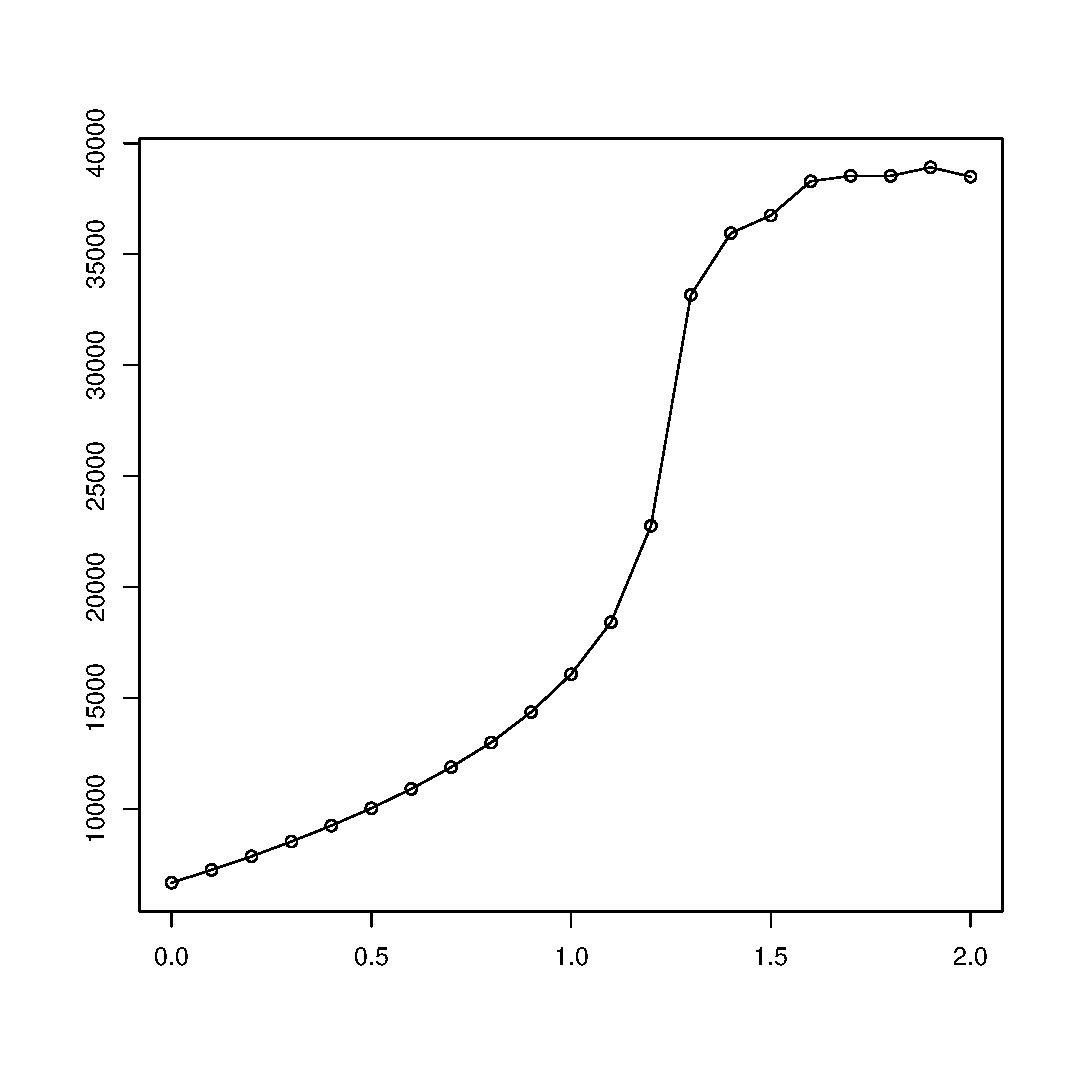
\includegraphics[width=8cm,height=6cm]{figures/pathsampling.eps}
\end{center}
\end{figure}

\footnotesize Approximation of $f(\beta)$ for the Potts model on
a $100\times 100$ image, a four-neighbor neighborhood, and $G=6$, based
on $1500$ MCMC iterations after burn-in.

\end{slide}\begin{slide}\slidetitle{Posterior Approximation (1)}

\begin{figure}[p!]
\begin{center}
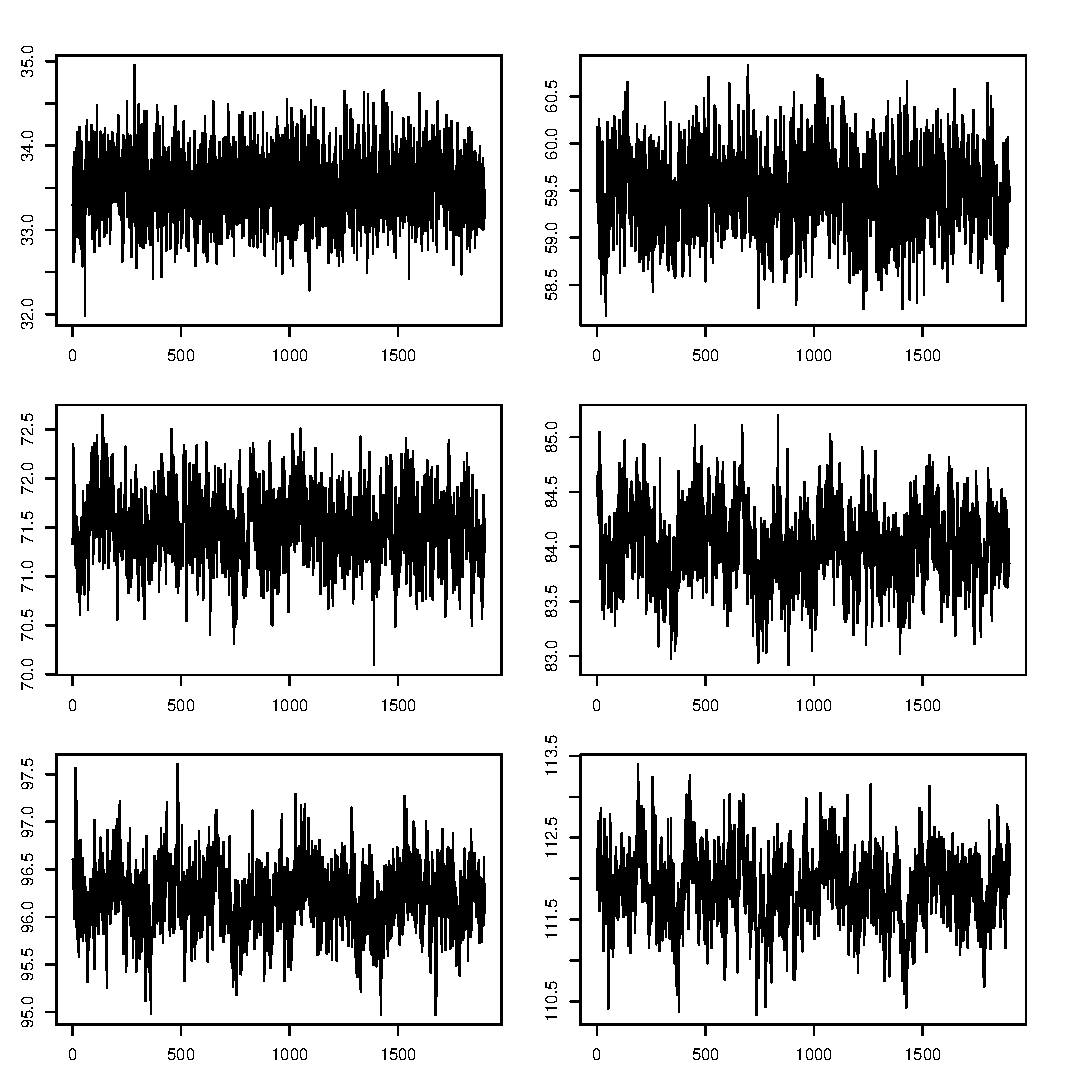
\includegraphics[width=10cm,height=5cm]{figures/mut.eps}
\end{center}
\end{figure}

\footnotesize Dataset {\sf Menteith}: Sequence of $\mu_g$'s based on $2000$ iterations of the hybrid Gibbs sampler ({\em read
row-wise from $\mu_1$ to $\mu_6$}).

\end{slide}\begin{slide}\slidetitle{Posterior Approximation (2)}

\begin{figure}[p!]
\begin{center}
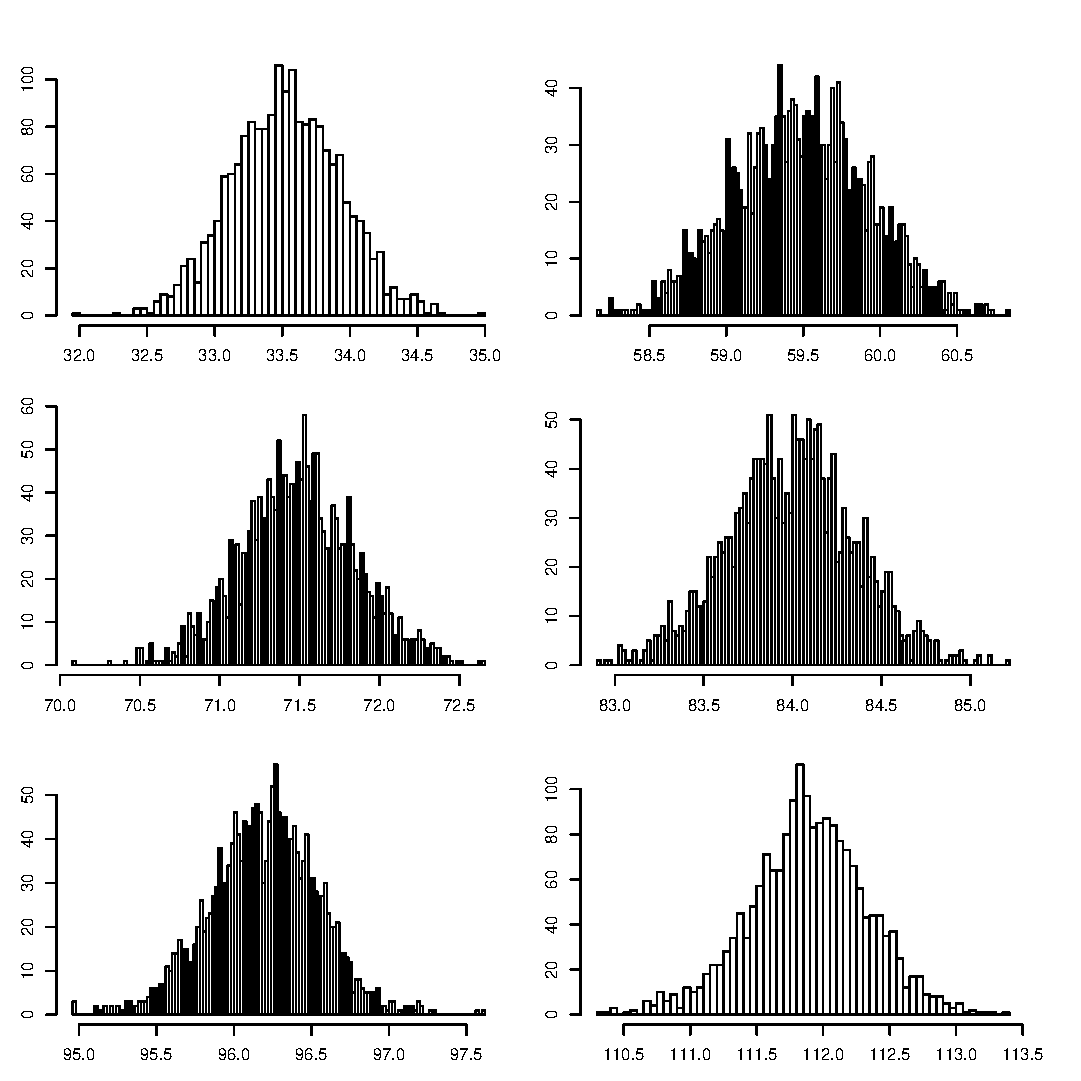
\includegraphics[width=6cm,height=5cm]{figures/muh.eps}
\end{center}
\end{figure}

\footnotesize Histograms of the $\mu_g$'s

\end{slide}\begin{slide}\slidetitle{Posterior Approximation (3)}

\begin{figure}
\begin{center}
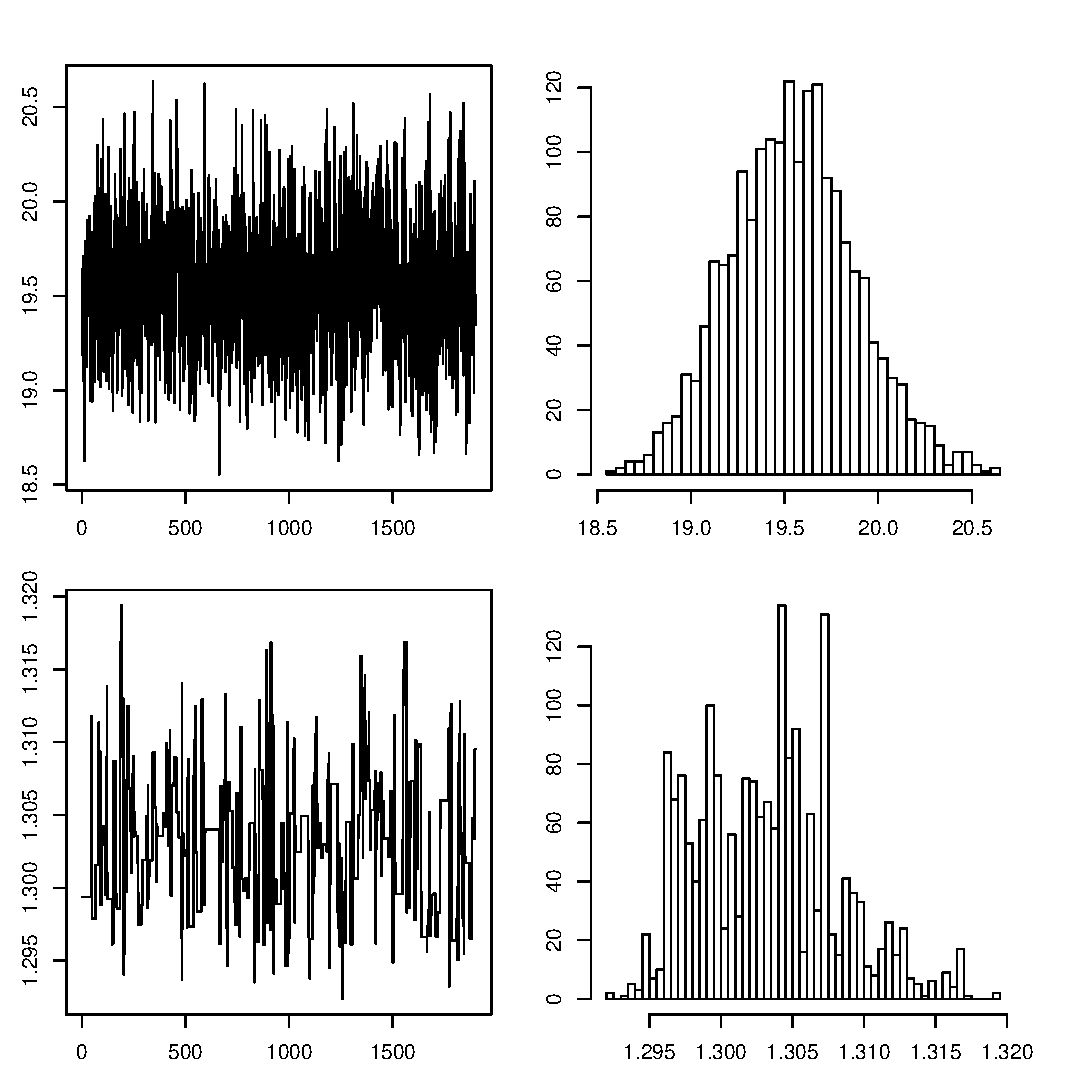
\includegraphics[width=6cm,height=5cm]{figures/betesig.eps}
\end{center}
\end{figure}

\footnotesize Raw plots and histograms of the $\sigma^2$'s and $\beta$'s based on $2000$
iterations of the hybrid Gibbs sampler

\end{slide}\begin{slide}\slidetitle{Image segmentation (1)}

Based on $(\bx^{(t)})_{1\le t\le T}$, an estimator of $\bx$ needs to be derived from an
evaluation of the consequences of wrong allocations. 

\vs \pause Two common ways corresponding to two loss functions
$$
L_1(\bx,\widehat\bx) = \sum_{i\in\mathcal{I}} \mathbb{I}_{x_i\ne\hat x_i},
$$
$$
L_2(\bx,\widehat\bx) =  \mathbb{I}_{\bx\ne\widehat\bx}\,,
$$

\vs \pause Corresponding estimators
$$
\hat x^{MPM}_i=\arg\max_{1\le g\le G} \mathbb{P}^\pi(x_i=g|\by)\,,\quad i\in\mathcal{I}\,,
$$
$$
\widehat\bx^{MAP} = \arg\max_{\bx} \pi(\bx|\by)\,,
$$

\end{slide}\begin{slide}\slidetitle{Image segmentation (2)}

\BrickRed{$\widehat\bx^{MPM}$ and $\widehat\bx^{MAP}$ not available in closed form!}

Approximation
$$
\hat x^{MPM}_i=\max_{g\in\{1,\ldots,G\}}\sum_{j=1}^N \mathbb{I}_{x_i^{(j)}=g}\,,
$$
based on a simulated sequence, $\bx^{(1)},\ldots,\bx^{(N)}$.

\end{slide}\begin{slide}\slidetitle{Image segmentation (3)}

\begin{figure}
\begin{center}
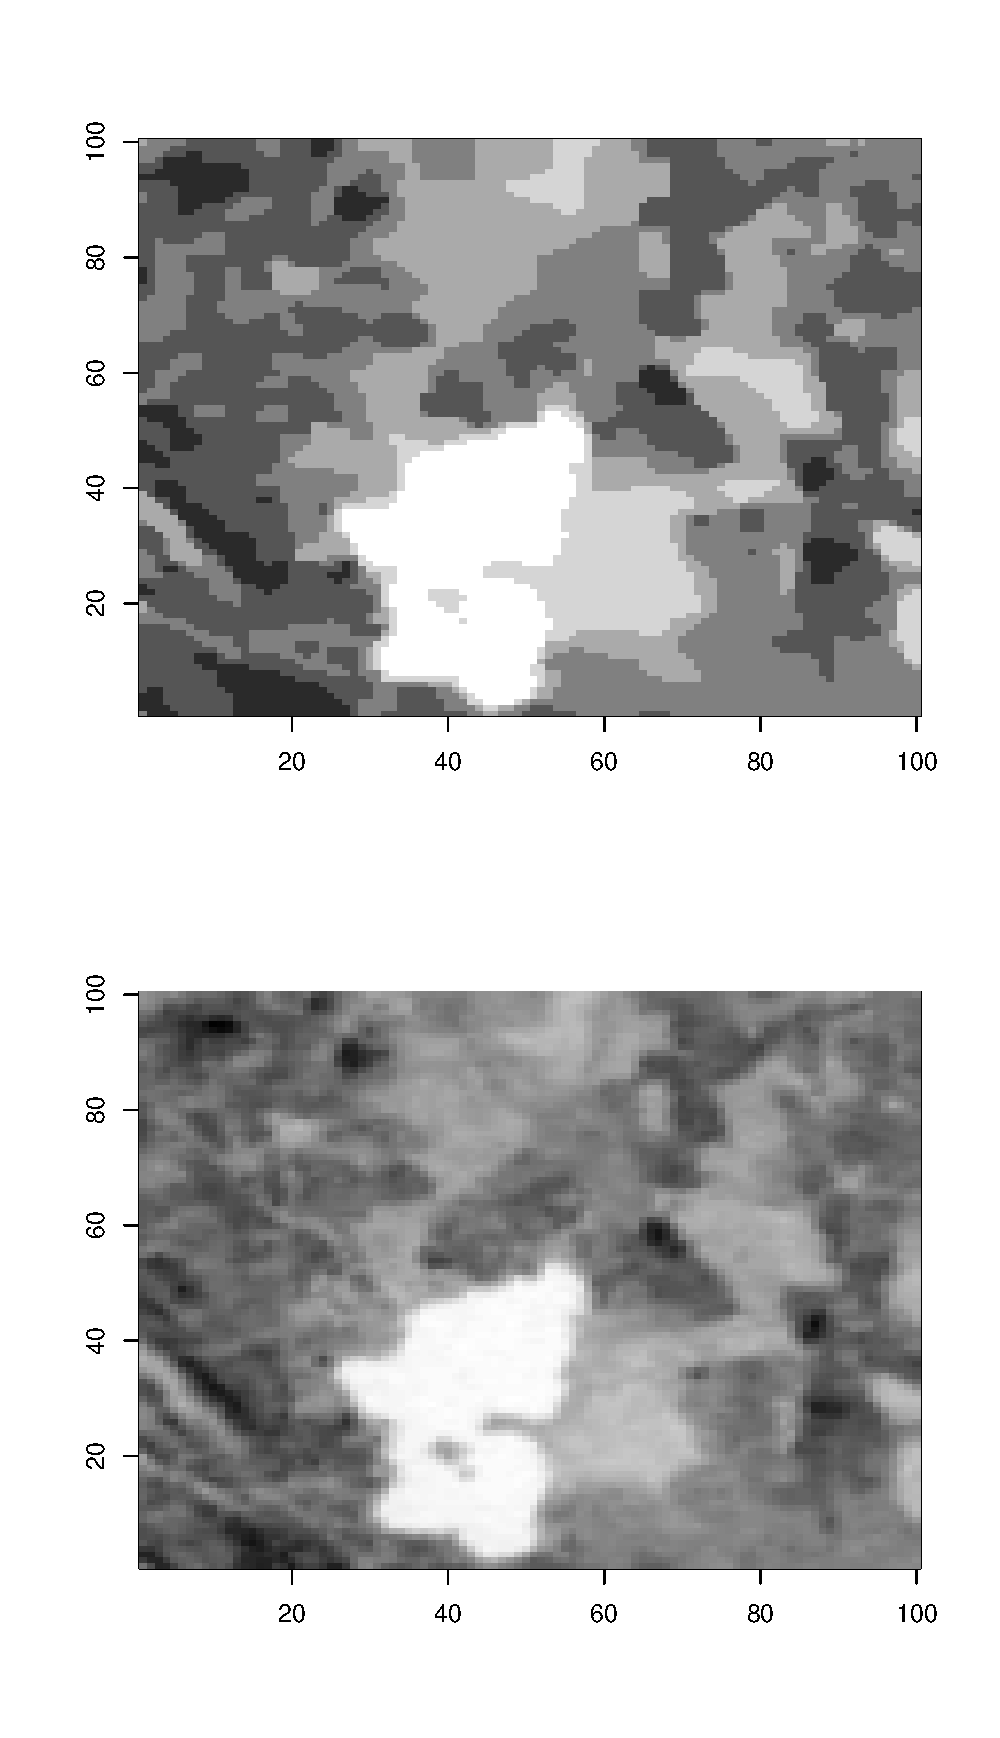
\includegraphics[width=5cm,height=6cm]{figures/recons.eps}
\end{center}
\end{figure}

\footnotesize ({\em top}) Segmented image based on the MPM estimate produced after $2000$ iterations of
the Gibbs sampler and ({\em bottom}) the observed image

\end{slide}
